\clearpage

\section{Generation of AWG Compatible Signals}

\begin{tcolorbox}	
\begin{tabular}{p{2.75cm} p{0.2cm} p{10.5cm}} 	
\textbf{Student Name}  &:& Francisco Marques dos Santos\\
\textbf{Starting Date} &:& September 1, 2017\\
\textbf{Goal}          &:& Convert simulation signals into waveform files compatible with the laboratory's Arbitrary Waveform Generator\\
Directory              &:& mtools
\end{tabular}
\end{tcolorbox}


This section shows how to convert a simulation signal into an AWG compatible waveform file through the use of a matlab function called sgnToWfm. This allows the application of simulated signals into real world systems.

\subsection{sgnToWfm}

[data, symbolPeriod, samplingPeriod, type, numberOfSymbols, samplingRate] = sgnToWfm(fname\_sgn, nReadr, fname\_wfm );

\subsection*{Inputs}

\indent

\textbf{fname\_sgn}: Input filename of the signal (*.sgn) you want to convert. It must be a real signal (Type: TimeContinuousAmplitudeContinuousReal).
\bigskip

\textbf{nReadr}: Number of symbols you want to extract from the signal.
\bigskip

\textbf{fname\_wfm}: Name that will be given to the waveform file.

\subsection*{Outputs}
A waveform file will be created in the Matlab current folder. It will also return six variables in the workspace which are:
\bigskip

\textbf{data}: A vector with the signal data.
\bigskip

\textbf{symbolPeriod}: Equal to the symbol period of the corresponding signal.
\bigskip

\textbf{samplingPeriod}: Sampling period of the signal.
\bigskip

\textbf{type}: A string with the name of the signal type.
\bigskip

\textbf{numberOfSymbols}: Number of symbols retrieved from the signal.
\bigskip

\textbf{samplingRate}: Sampling rate of the signal.


\subsection*{Functional Description}

This matlab function generates a *.wfm file given an input signal file (*.sgn). The waveform file is compatible with the laboratory's Arbitrary Waveform Generator (Tekatronix AWG70002A). In order to recreate it appropriately, the signal must be real, not exceed $8*10^9$ samples and have a sampling rate equal or bellow 16 GS/s.


\subsection*{This function can be called with one, two or three arguments:}
Using one argument:

\bigskip

\noindent
[data, symbolPeriod, samplingPeriod, type, numberOfSymbols, samplingRate] = sgnToWfm('S6.sgn');
\bigskip

\noindent
This creates a waveform file with the same name as the *.sgn file and uses all of the samples it contains.
\bigskip

\noindent
Using two arguments:

\bigskip

\noindent
[data, symbolPeriod, samplingPeriod, type, numberOfSymbols, samplingRate] = sgnToWfm('S6.sgn',256);
\bigskip

\noindent
This creates a waveform file with the same name as the signal file name and the number of samples used equals nReadr x samplesPerSymbol. The samplesPerSymbol constant is defined in the *.sgn file.
\bigskip

\noindent
Using three arguments:

\bigskip

\noindent
[data, symbolPeriod, samplingPeriod, type, numberOfSymbols, samplingRate] = sgnToWfm('S6.sgn',256,'myWaveform.wfm');
\bigskip

\noindent
This creates a waveform file with the name "myWaveform" and the number of samples used equals nReadr x samplesPerSymbol. The samplesPerSymbol constant is defined in the *.sgn file.

\subsection{Loading a signal to the Tekatronix AWG70002A}

The AWG we will be using is the Tekatronix AWG70002A which has the following key specifications:
\bigskip

\textbf{Sampling rate up to 16 GS/s}: This is the most important characteristic  because it determines the maximum sampling rate that your signal can have. It must not be over 16 GS/s or else the AWG will not be able to recreate it appropriately.
\bigskip

\textbf{8 GSample waveform memory}: This determines how many data points your signal can have.
\bigskip

After making sure this specifications are respected you can create your waveform using the function. When you load your waveform, the AWG will output it and repeat it constantly until you stop playing it.
\bigskip

\textbf{1. Using the function sgnToWfm}:
Start up Matlab and change your current folder to mtools and add the signals folder that you want to convert to the Matlab search path. Use the function accordingly, putting as the input parameter the signal file name you want to convert.
\bigskip

\noindent
\textbf{2. AWG sampling rate}:
After calling the function there should be waveform file in the mtools folder, as well as a variable called samplingRate in the Matlab workspace. Make sure this is equal or bellow the maximum sampling frequency of the AWG (16 GS/s), or else the waveform can not be equal to the original signal. If it is higher you  have to adjust the parameters in the simulation in order to decrease the sampling frequency of the signal(i.e. decreasing the bit period or reducing the samples per symbol).
\bigskip

\noindent
\textbf{3. Loading the waveform file to the AWG}:
Copy the waveform file to your pen drive and connect it to the AWG. With the software of the awg open,go to browse for waveform on the channel you want to use, and select the waveform file you created (Figure 7.1).

\begin{figure}[h]
	\centering
	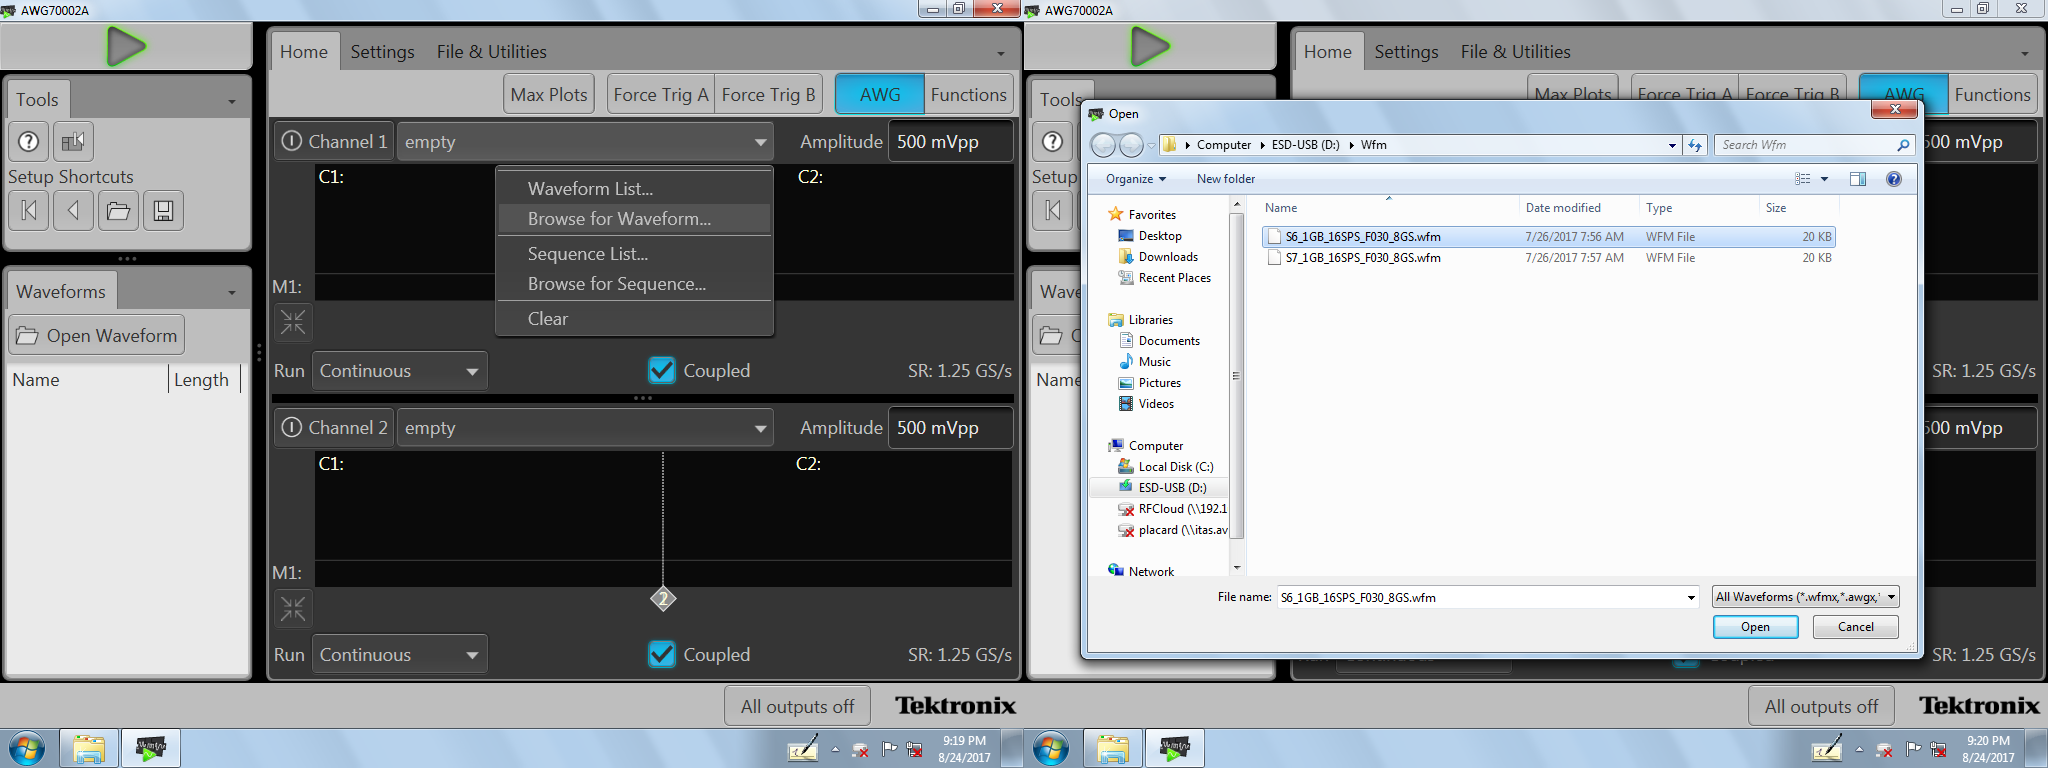
\includegraphics[width=10cm]{../mtools/sgnToWfm/figures/tutorial1}
	\label{TUT_SelectingWFM}\caption{Selecting your waveform in the AWG}
\end{figure}
\begin{figure}[h]
	\centering
	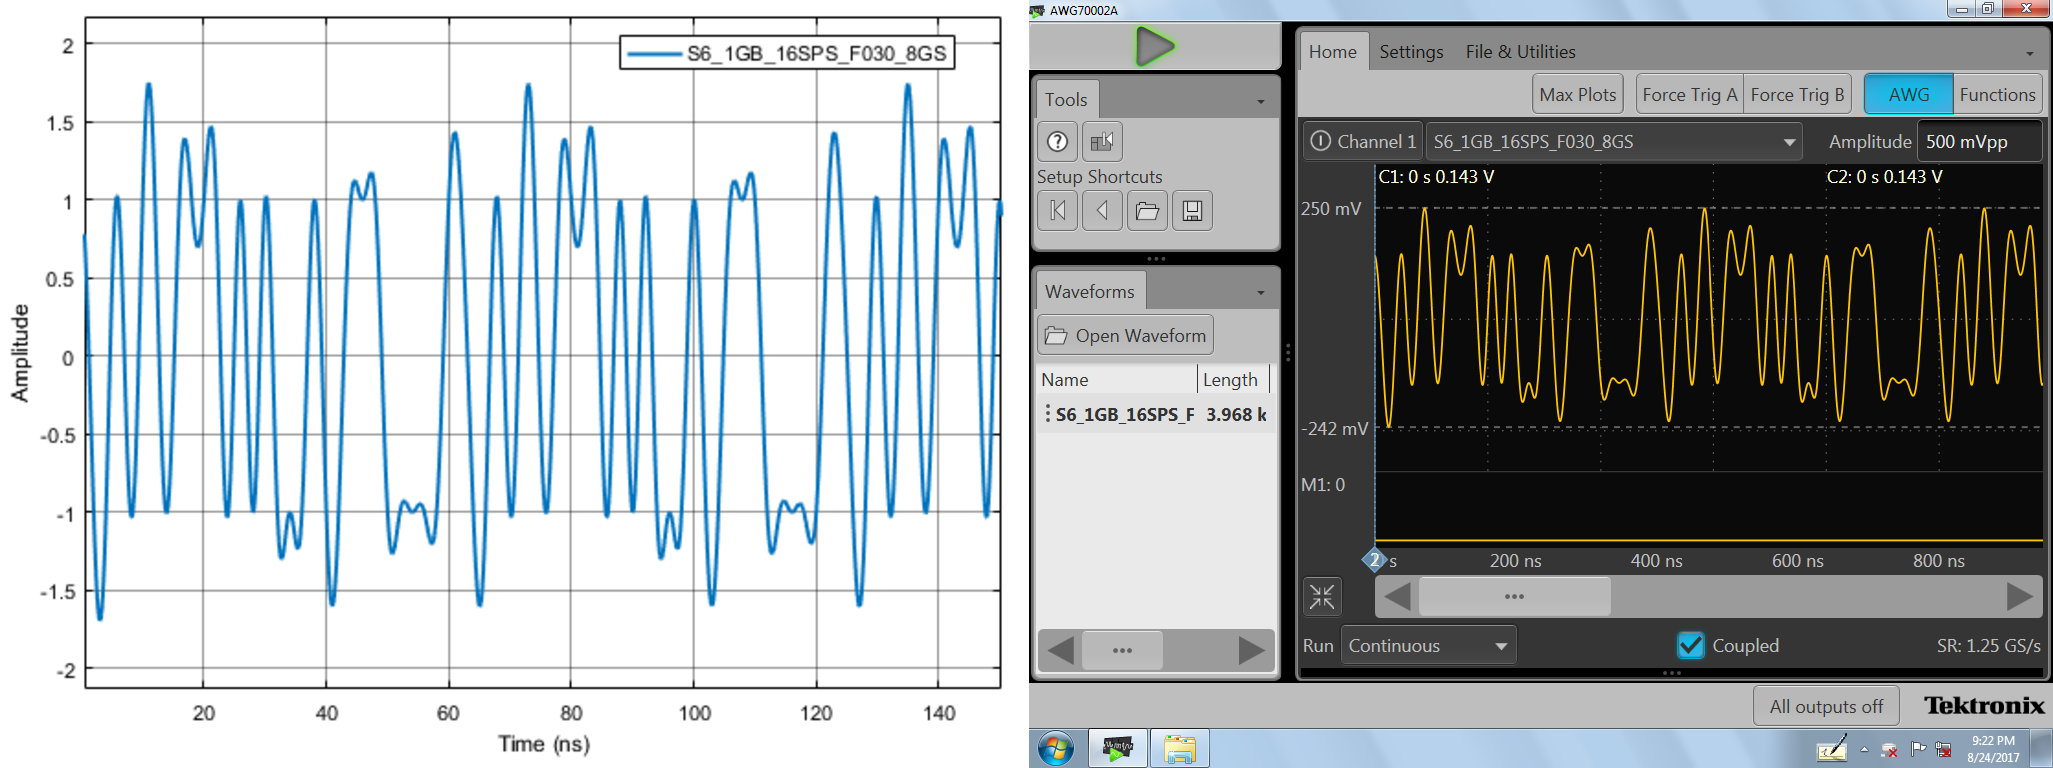
\includegraphics[width=10cm]{../mtools/sgnToWfm/figures/tutorial2}
	\label{TUT_CompBad}\caption{Comparison between the waveform in the AWG and the original signal before configuring the sampling rate}
\end{figure}

Now you should have the waveform displayed on the screen. Although it has the same shape,  the waveform might not match the signal timing wise due to an incorrect sampling rate  configured in the AWG.
In this example (Figure 7.2), the original signal has a sample rate of 8 GS/s and the AWG is configured to 1.25 GS/s. Therefore it must be changed to the correct value.
To do this go to the settings tab, clock settings, and change the sampling rate to be equal to the one of the original signal, 8 GS/s (Figure 7.3).
\begin{figure}[h]
	\centering
	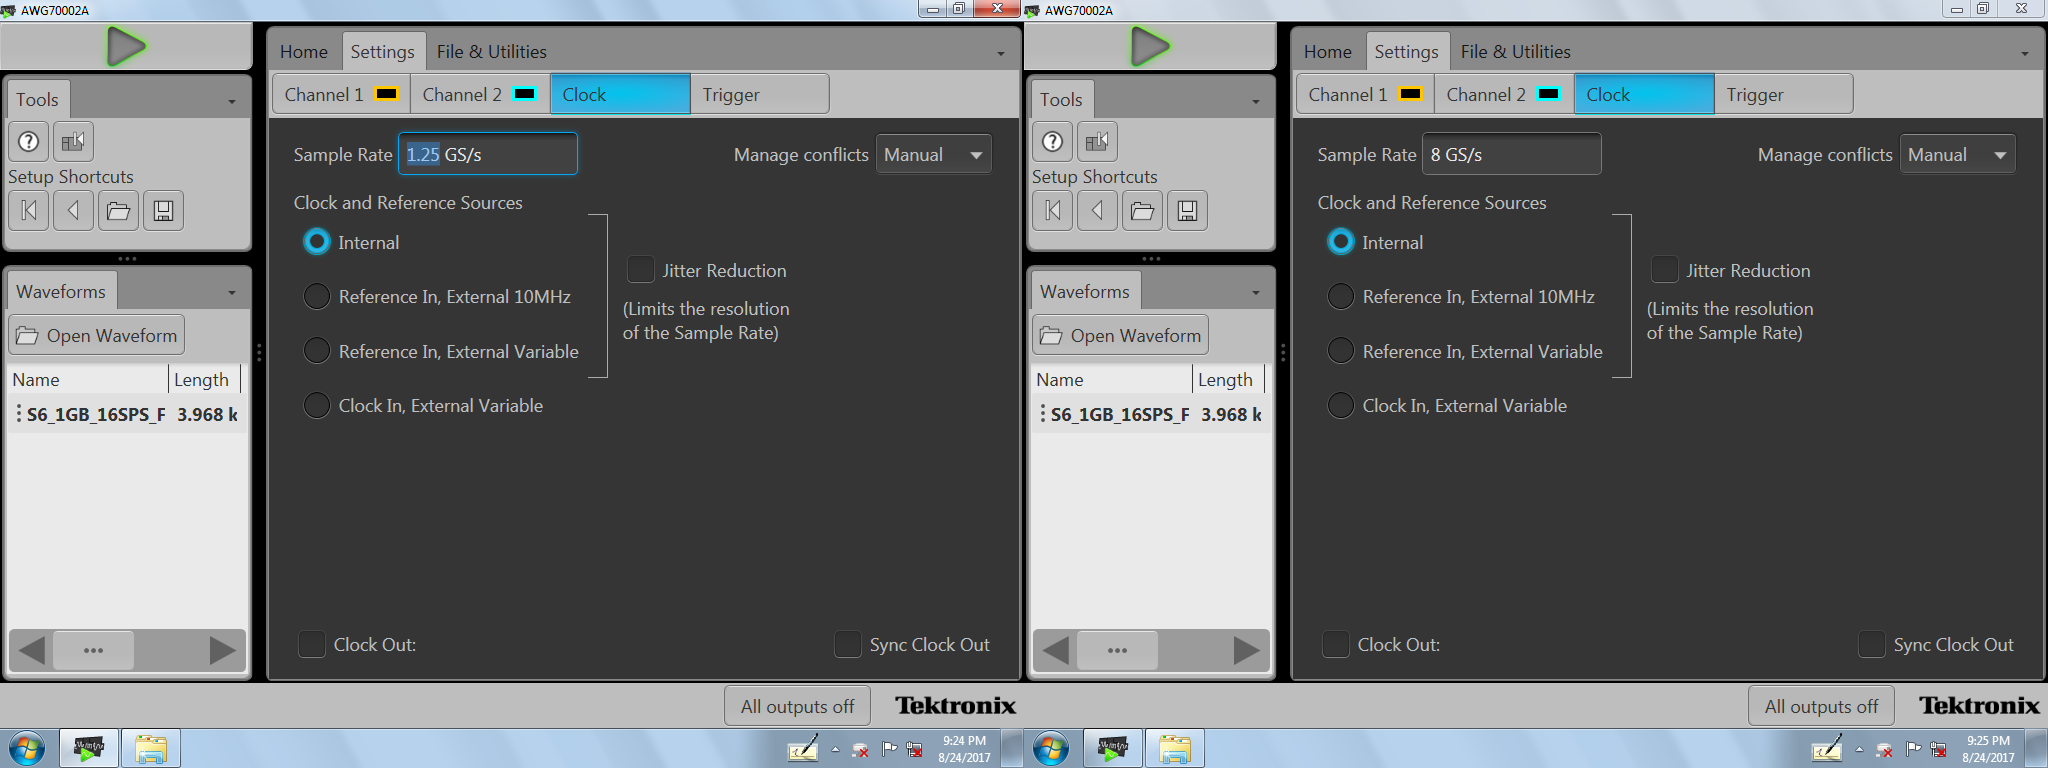
\includegraphics[width=10cm]{../mtools/sgnToWfm/figures/tutorial3}
	\label{TUT_ConfigSR}\caption{Configuring the right sampling rate}
\end{figure}
Compare the waveform in the AWG with the original signal, they should be identical (Figure 7.4).
\begin{figure}[h]
	\centering
	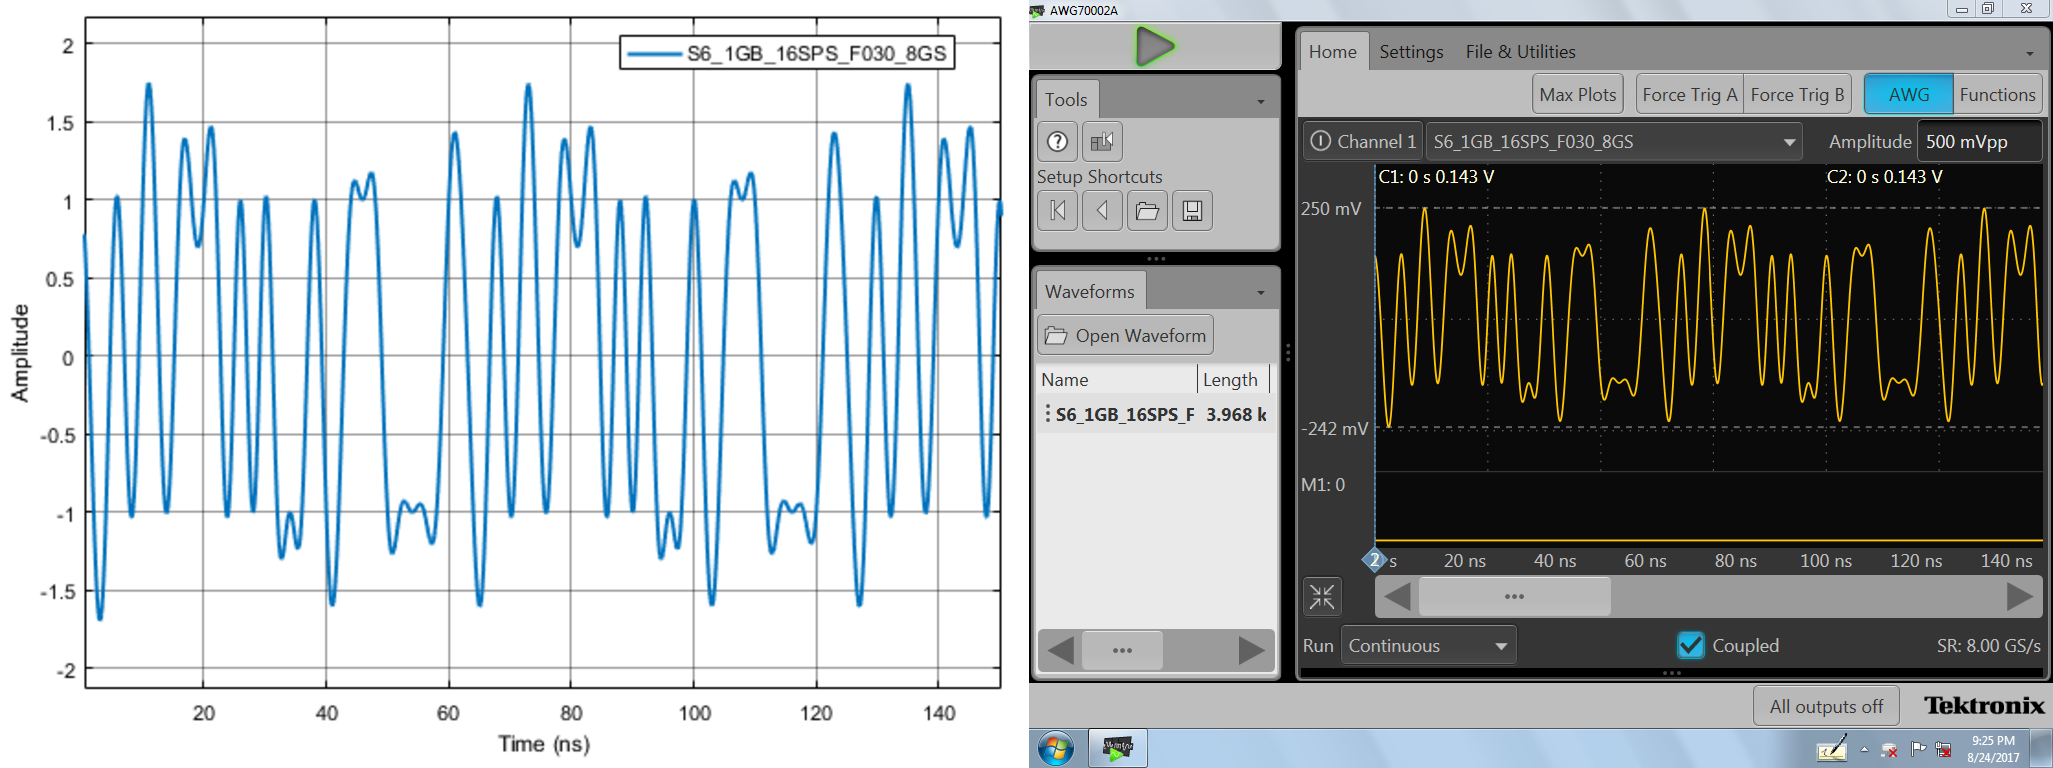
\includegraphics[width=10cm]{../mtools/sgnToWfm/figures/tutorial4}
	\label{TUT_CompGood}\caption{Comparison between the waveform in the AWG and the original signal after configuring the sampling rate}
\end{figure}
\bigskip

\noindent
\textbf{4. Generate the signal}:
Output the wave by enabling the channel you want and clicking on the play button.


%\end{document} 